
\begin{itemize}
    \item \textsc{Model} : Describe real world problem with
        \begin{itemize}
            \item \textbf{Variables} : $X = \{x_1, x_2,\cdots, x_n\}$

            \item \textbf{Domains} : $D = \{ D(x_1), D(x_2),\cdots,
                D(x_n)\}$

                \begin{itemize}
                    \item[Ex:] Booleans, \textbf{finite domains}, finite
                        set, intervals, continuous domains,\ldots
                \end{itemize}
            \item \textbf{Constraints} : $C = \{c_1, c_2,\cdots, c_e\}$
                \begin{itemize}
                    \item A \textbf{scope} $\scp(c) = (x_1, x_2,\cdots,x_{r_e})$ : is the
                        variables constrained by c.
                    \item A \textbf{relation} $\rel(c)$ : value combinations accepted by
                        c
                \end{itemize}

                \begin{tabular}{m{1.5cm}m{12cm}}
                    Used for:&
                \begin{enumerate}
                    \item Feasibility checking: Check if the constraint can be satisfied
                        given it's variables domain. 

                    \item Pruning: remove values from the domains if they do not appear
                        in any solution of the constraint.
                \end{enumerate}
                \end{tabular}

            \item \textbf{Objective function} : $O : \sol \to \R$
        \end{itemize}

        \paragraph{Types}
        \begin{enumerate}
            \item CSP${} = (X, D, C)$
            \item COP${} = (X, D, C, O)$
        \end{enumerate}

        \paragraph{Declarative} : describe what you want not how to get it

    \item \textsc{Search} : Describe how to solve the problem and
        explore the search space
        \begin{itemize}
            \item \textbf{Propagation} : Use constraints to remove
                \textit{useless} (doesn't remove solution) parts of the
                search space. It's a filtering where we remove
                value from non feasible solutions.
                \begin{center}
                    \scriptsize
                    \textit{Need choice between more pruning with more
                        expensive to compute or less proning cheaper to
                    compute}
                \end{center}

                \begin{itemize}
                    \item Consistencies : Require that all the values
                        are able to satisfy their constaints in
                        \textbf{isolation}

                    \item Propagator: used at the beginning of the search
                        and each time a decision is made.
                \end{itemize}
            \item \textbf{Backtracking Tree Search} : Explore search
                space by taking decisions and backtracking (with
                remembering decision)

                \paragraph{Current node}: The node is modified at each decision
                made and it is restored when backtracking occurs.
        \end{itemize}

        \paragraph{Search space} = $D(x_1) \times D(x_2) \times \cdots \times D(x_n)$
\end{itemize}

The communication between the Constraints and the Search is done through the domain of the variables in CP.
When a constraint modify the domain, it is called \emph{propagation} and when it is the search it is called \emph{branching}.


\subsection{Pruning}

\subsubsection{Fix-point algorithm}

\begin{lstlisting}
repeat
    select a constraint c
    if c is OK wrt the domain store
        apply pruning algorithm of c
    else
        return KO
until no value can be removed
\end{lstlisting}

\begin{tabular}{m{8cm}cm{8cm}}
    %TODO tikz
    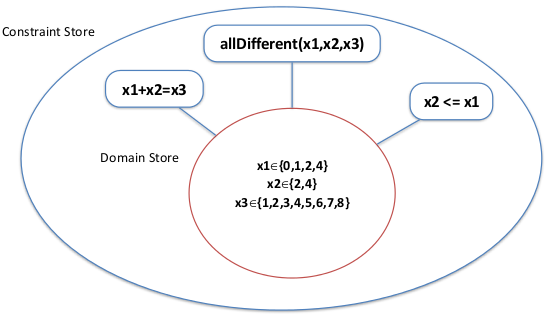
\includegraphics[width=8cm]{fixPoint1}
    & $\Rightarrow$ &
    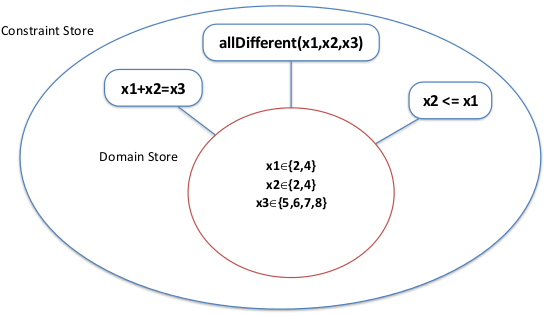
\includegraphics[width=8cm]{fixPoint2}
\end{tabular}


\subsection{Consistency}

\begin{itemize}
    \item A CSP (\textsc{X, D, C}) is $X_{Consistent}$ iff all
        constraints $c \in C$ are $X_{Consistent}$ ($X_{Consistent}$ is
        GAC, BC,\ldots)

    \item A consistency $S_1$ is stronger than a consistency $S_2$ iff all CSP respecting
        $S_1$ also respect $S_2$.

        Note that some consistencies can be \textit{incomparable}

        \begin{center}
            \begin{tabular}{l|c|c|}
                \cline{2-3}
                \multirow{1}{*}{
                    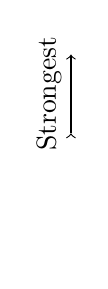
\begin{tikzpicture}
                        \node (0,0) {};
                        \draw[->] (0,1.5) edge node [left]{\rotatebox{90}{Strongest}}
                        (0, 2.5);
                \end{tikzpicture}} 
                &
                \multicolumn{2}{c|}{GAC} \\
                \cline{2-3}
                & Bound consistency & Forward checking \\
                \cline{2-3}
            \end{tabular}
        \end{center}

        This is a tradeoff between \textbf{Speed} and \textbf{Filtering}.

\end{itemize}


\subsubsection{Filtering consistencies}

if $x$ is a domain filtering consistency, a propagator for $x$ will :
from CSP(X, D, X)
\begin{itemize}
    \item return (X, D', C) such that
        \begin{itemize}
            \item D' $\subseteq$ D
            \item (X, D, C) and (X, D', C) equivalent
            \item D' is a nonempty partial solution
            \item (X, D', C) respect $x$
        \end{itemize}
    \item return \textcolor{red}{fail} if no such CSP exists.

        $\to$ not possible to satisfy consistency = unsatisfiable CSP
\end{itemize}

\begin{itemize}
    \item \textbf{Arc consistency} (also called domain consistency):
        every value of every variable participates in a solution of the
        constraint, so all value of variables are \textbf{supported}.

        \begin{tabular}{m{1cm}m{13cm}}
            Note:&
        \begin{itemize}
            \item It's the strongest filtering when considering constraints in isolation.
                \item  GAC $\neq$ satisifability :i A CSP that is GAC may not
        be satisfiable.
        \end{itemize}
        \end{tabular}

        \paragraph{GAC} A constraint $c$ is GAC iff
        \begin{lstlisting}[mathescape]
$\forall x_i \in scope(c)$
    $\forall a_i \in D(x_i)$
        $\exists a_1,..., a_{i-1}, a_{i+1},..., a_r \in D(x_1) \times ... \times D(x_{i-1}) \times D(x_{i+1}) \times ... \times D(x_r)$ such that $(a_1,...,a_r) \in c$
        \end{lstlisting}


    \item \textbf{Bound consistency}: assuming domains are intervals,
        every bound of every variable participates in a solution of the
        constraint.

        \begin{itemize}
            \item GAC can be costly, so a other consistency is to
                only search support for bound.
            \item[$\to$] all valuyes between min and max considered in the domain.
        \end{itemize}


        \paragraph{BC} A constraint $c$ is BC iff
        \begin{lstlisting}[mathescape]
$\forall x_i \in scope(c)$
    $\forall a_i \in \{ \quad min(D(x_i)), max(D(x_i))\quad \}$
        $\exists a_1,..., a_{i-1}, a_{i+1},..., a_r  \in D*(x_1) \times ... \times D*(x_{i-1}) \times D*(x_{i+1}) \times ... \times D*(x_r):$ such that $c(a_1,..., a_r)$

$D*(x_k) = [min(D(x_k)), max(D(x_k))]$
        \end{lstlisting}


    \item \textbf{Forward checking}

        It's like a GAC at the end.

        \paragraph{FC} A constraint $c$ is FC iff
        \begin{lstlisting}[mathescape]
if $\forall x_i \in scope(c):$ $D(x_i) = \{v_i\}$ then $c(v_1, ..., v_r)$
if all but one variable assigned: $c$ is GAC
        \end{lstlisting}
\end{itemize}



\subsection{Global constraints}

\paragraph{Advantage}
\begin{itemize}
    \item Increasing expressivity of CP
    \item Pruning strength because the propagation considered constraint in isolation
        but global constraint is like \textbf{a set of constraint}
    \item Pruning efficiency because no fixed point between small constraints
        but a more flobal reasoning
\end{itemize}

\subsubsection{Decomposition}
A set of constraints $S$ is called the decomposition of $g$ iff :
$$ \forall D(X): sols(X, D(X), \{g\}) = sols(X, D(X), S)$$

\begin{itemize}
\item GAC pruning equivalent in $S$ and $g$ iff the constraint
graph of the D is \textbf{acyclic}.

Otherwise, GAC pruning stronger in global constraint

\begin{itemize}
    \item GAC on decomposition : supports(s) for each literal on each constraints
        \textbf{separately}
    \item GAC on global constraint: global support(s) for each literal on global constraint
\end{itemize}


\item FC pruning stronger in the decomposition
    \end{itemize}



\subsubsection{AllDifferent constraint}

GAC pruning for \texttt{allDifferent($[x_1,\cdots, x_r]$)} use a value graph :
\begin{itemize}
    \item one node for each variable $x_1,\cdots, x_r$
    \item one node for each value in $\cap D(x_i)$
    \item one edge between $x_i$ and $a$ if $a \in D(x_i)$
    \item[Note:] bipartite graph
\end{itemize}

\paragraph{Matching}
A matching is a \textbf{set of edgges} such that no edge share
a same node.

\begin{itemize}
    \item Size matching = \# edges
    \item Maximum matching = largest size
    \item Maximum size = \# variables
\end{itemize}

\begin{description}
    \item \texttt{AllDifferent($[x_1,\cdots, x_r]$)} satisifiable iff
        $\exists$ matching of the value graph covering $x_1,\cdots, x_r$ (=
        matching of maximum size)
    \item M is a maximum matching iff no augmenting
        path exists
\end{description}

\paragraph{Finding a maximum matching}

\begin{enumerate}
    \item Start with any matching (e.g. empty matching)
    \item Iteratively improve the matching with \textbf{augmenting path}

        \paragraph{Augmenting path}
        \begin{itemize}
            \item Edge in M : variables $\to$ values
            \item Other : values $\to$ variables

            \item[$\Rightarrow$] An augmenting path is a \textbf{directed path}
                from a uncovered value to an uncovered variable.

                Use DSF or BFS
        \end{itemize}

        \begin{figure}[!h]
            \centering
            %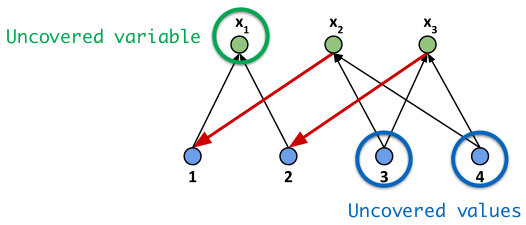
\includegraphics[width=8cm]{img/augmenting-paths.png}
            \caption{Augmenting paths}
        \end{figure}

    \item Stop when no more augmenting paths
\end{enumerate}

\paragraph{GAC}

\begin{description}
    \item \texttt{AllDifferent} is \textbf{GAC} iff all edge belong to
        a maximun matching covering all the variables
\end{description}

\begin{itemize}
    \item \textbf{Alternating path}

    \item \textbf{Alternating cycle}

\end{itemize}

\paragraph{Filtering}

\begin{enumerate}
    \item Find a maximun matching M
    \item if M.size != \#variables : \textcolor{red}{Fail}

    \item Find all edges belonging to an even \textbf{length alternating
        path} startint at a uncovered node (DFS or BDS)

        \paragraph{Alternating path}: start at an uncovered node and
        switch the edges in/out the matching. Change values
        of variables to stays maximum with different edges.

        \begin{figure}[!h]
            \centering
            %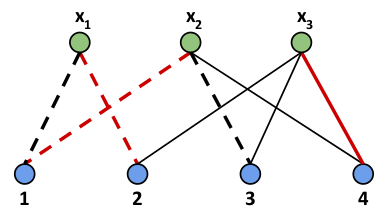
\includegraphics[width=8cm]{img/alternating.png}
            \caption{Alternating paths}
        \end{figure}

    \item Find all edges belonging to \textbf{alternating cycle} which
        correpons to the strongly connected components in the directed value
        graph

        \paragraph{Alternating cycle}: switch the edges in/out the matching.
        Exchange values of variables to stays maximum with different edges.

    \item Remove all edges/literals not in M and not found
\end{enumerate}

\paragraph{Incrementality of the filtering}
The value graph and maximum matching is keep in memory between calls to propagator.

\begin{tabular}{cm{12cm}}
When called
&
\begin{enumerate}
    \item Remove esdge not present anymore
    \item recompute maximum matching if necessary
    \item recompute GAC edges
\end{enumerate}
\end{tabular}

\subsubsection{Sum constraint}

\paragraph{NP-Hard}
Gac for a sum constraint is NP-Hard :

\paragraph{Proof} reduction of subset-sum to GAC for Sum
\begin{itemize}
    \item subset-sum: a NP-Hard problem for integer set ($S=\{a_1,\cdots, a_r\}$),
        does any non-empty subset of S sums to 0?

    \item reduction to GAC for Sum:
        \begin{lstlisting}[mathescape]
variables  $x_i$ with domains $\{0, a_i\}$
GAC on sum($[x_1,..., x_r], 0$)

if $D(x_i) = \{0\} \forall x_i$ : answer no
else: answer yes
\end{lstlisting}
\end{itemize}

\paragraph{Consequences} GAC propagator for sum is exponential (unless P=NP), so
the propagator is usually done with \textbf{Bound Consistency}

\paragraph{Bound consistency}

\begin{lstlisting}[mathescape]
propagate(){
    $\Delta = \emptyset$
    for( x $\leftarrow$ scope) {
        new_min = k - ($\sum_{(y \in scope, y \neq x)} y.max$)
        for( a $\leftarrow$ D(x) if a < new_min)
            $\Delta$ += (x, a)

        new_max = k - ($\sum_{(y \in scope, y \neq x)} y.min$)
        for( a $\leftarrow$ D(x) if a > new_max)
            $\Delta$ += (x, a)
    }
    return $\Delta$
}
\end{lstlisting}

\subsubsection{Element constraint}
%TODO

%TODO constraint slide 63 to 66



\subsection{Search}

CP mainly use DFS and at each
%TODO from slide 67 to the end











\subsection{Advantage}
\begin{itemize}
    \item Rich modeling language:
        \begin{itemize}
            \item  integer variables, set variables, graph variables
            \item  library of constraints (not necessarily linear)
        \end{itemize}
    \item  Fast prototyping
    \item  Easy to adapt/change a model
    \item  Extensible (you can create new constraints)
    \item  Great framework to hybridize with other techniques
\end{itemize}


